%%%%%%%%%%%%%%%%%%%%%%%%%%%%%%%%%%%%%%%%%
% Large Colored Title Article
% LaTeX Template
% Version 1.1 (25/11/12)
%
% This template has been downloaded from:
% http://www.LaTeXTemplates.com
%
% Original author:
% Frits Wenneker (http://www.howtotex.com)
%
% License:
% CC BY-NC-SA 3.0 (http://creativecommons.org/licenses/by-nc-sa/3.0/)
%
%%%%%%%%%%%%%%%%%%%%%%%%%%%%%%%%%%%%%%%%%

%----------------------------------------------------------------------------------------
%	PACKAGES AND OTHER DOCUMENT CONFIGURATIONS
%----------------------------------------------------------------------------------------

\documentclass[DIV=calc, paper=a4, fontsize=11pt, twocolumn]{scrartcl}	 % A4 paper and 11pt font size

\usepackage{multirow}
\usepackage{graphicx}
\usepackage[english]{babel} % English language/hyphenation
\usepackage[protrusion=true,expansion=true]{microtype} % Better typography
\usepackage{amsmath,amsfonts,amsthm} % Math packages
\usepackage[dvipsnames, svgnames,table]{xcolor} % Enabling colors by their 'svgnames'
\usepackage[hang, small,labelfont=bf,up,textfont=it,up]{caption} % Custom captions under/above floats in tables or figures
\usepackage{subcaption}
\usepackage{booktabs} % Horizontal rules in tables
\usepackage{fix-cm}	 % Custom font sizes - used for the initial letter in the document

\usepackage{sectsty} % Enables custom section titles
\allsectionsfont{\usefont{OT1}{phv}{b}{n}} % Change the font of all section commands

%\usepackage{fancyhdr} % Needed to define custom headers/footers
%\pagestyle{fancy} % Enables the custom headers/footers
%\usepackage{lastpage} % Used to determine the number of pages in the document (for "Page X of Total")

% Headers - all currently empty
%\lhead{}
%\chead{}
%\rhead{}

% Footers
%\lfoot{}
%\cfoot{}
%\rfoot{\footnotesize Page \thepage\ of \pageref{LastPage}} % "Page 1 of 2"

%\renewcommand{\headrulewidth}{0.0pt} % No header rule
%\renewcommand{\footrulewidth}{0.4pt} % Thin footer rule

\usepackage{lettrine} % Package to accentuate the first letter of the text
\newcommand{\initial}[1]{ % Defines the command and style for the first letter
\lettrine[lines=3,lhang=0.3,nindent=0em]{
\color{DarkGoldenrod}
{\textsf{#1}}}{}}

%----------------------------------------------------------------------------------------
%	TITLE SECTION
%----------------------------------------------------------------------------------------

\usepackage{titling} % Allows custom title configuration


\newcommand\prob{$n$-People $k$-Bikes Problem}
\newcommand\Prob{\prob}

\newcommand{\HorRule}{\color{DarkGoldenrod} \rule{\linewidth}{1pt}} % Defines the gold horizontal rule around the title

\pretitle{\vspace{-30pt} \begin{flushleft} \HorRule \fontsize{32}{32} \usefont{OT1}{phv}{b}{n} \color{DarkRed} \selectfont} % Horizontal rule before the title

\title{The \Prob} % Your article title

\posttitle{\par\end{flushleft}\vskip 0.5em} % Whitespace under the title

\preauthor{\begin{flushleft}\large \lineskip 0.5em \usefont{OT1}{phv}{b}{sl} \color{DarkRed}} % Author font configuration

\author{Lancer \r{A}ngstr\"{o}m, } % Your name

\postauthor{\footnotesize \usefont{OT1}{phv}{m}{sl} \color{Black} % Configuration for the institution name
Dept. for Biologically-Impelled Konveyance and Excursion Research Studies% Your institution

\par\end{flushleft}\HorRule} % Horizontal rule after the title

\date{} % Add a date here if you would like one to appear underneath the title block

%----------------------------------------------------------------------------------------

\begin{document}

\maketitle % Print the title

%\thispagestyle{fancy} % Enabling the custom headers/footers for the first page 

%----------------------------------------------------------------------------------------
%	ABSTRACT
%----------------------------------------------------------------------------------------

% The first character should be within \initial{}
%\initial{H}\textbf{ere is some sample text to show the initial in the introductory paragraph of this template article. The color and lineheight of the initial can be modified in the preamble of this document.}

\initial{W}e present and solve the {\em \prob}. This problem concerns a group of $n$ people who possess among them $k$ bikes, with $k<n$, and wish to travel to a destination $d$ in a way that minimizes the time it takes the last member among them to arrive. We show that $n$ people can, indeed, use $k$ bikes to accelerate their travel beyond walking speed, and give an algorithm for planning bicycle allocation for general $n$ and $k$.

The \prob~has far-reaching implications in many fields, including comestibility theory~\cite{comestibility}, deep-space navigation~\cite{arkanoid}, maximum-jerk motion planning~\cite{jerk2}, and pop-math brainteasers.


%----------------------------------------------------------------------------------------
%	ARTICLE CONTENTS
%----------------------------------------------------------------------------------------
\section{Introduction}

\initial{Y}ou're hungry. Your $n-1$ friends, some of whom are cyclists, are also hungry. Collectively, you decide to venture out from the comfort of your respective offices on campus, through the perilously cold (and often wet) outdoors of the Pittsburgh winter, to your favorite dining establishment $d$.\footnote{
We have only experimentally verified our research in the specific case of $d =$ {\sf Chipotle}, though we expect the results to generalize to all $d$.}
During the journey, however, the advancing hunger and tormenting weather overcome your group's desire to amble idly at the leisurely walking speed of $w$.
You glance over at your cyclist friends, who are pushing along their $k$ bikes beside themselves, and wonder: ``Might there be a way to exploit the bikes so that all $n$ of us can get to $d$ sooner?''

Such is the {\em \prob}.

\section{Problem Statement}

\begin{figure}[h]
	\begin{center}
	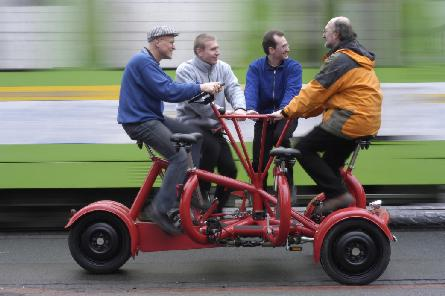
\includegraphics[width=0.5\textwidth]{conference.jpg}
	\end{center}
	\caption{Not like this.}
	\label{fig:conference}
\end{figure}
\begin{figure}[h]
	\begin{center}
	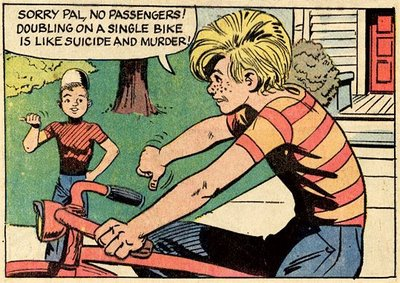
\includegraphics[width=0.5\textwidth]{suicideandmurder.jpg}
	\end{center}
	\caption{Stripe-Boy demonstrates correct bicycle allocation protocol. (Helmets are apparently beyond the scope of his work.)}
	\label{fig:stripey}
\end{figure}

{T}he precise formulation and constraints of the problem are as follows.
\initial{G}iven $n$ people and $k$ bikes, $n<k$, all colocated, where:
\begin{enumerate}
	\setlength{\itemsep}{-0.5em}
	\item each person can travel on foot, at walking speed $w$, or bike at speed $b$, with $w<b$,
	\item mounting and dismounting a bike takes a negligible amount of time $\epsilon$,
	\item at most one person can ride a given bike at a time (see Figures~\ref{fig:conference} and \ref{fig:stripey}), and
	\item bikes are stationary when not ridden,
\end{enumerate}

show how all $n$ people can arrive at a destination $d$ in some time $t$ {\em less} than that afforded by walking speed $w$.\footnote{So ``$k$ people bike the entire distance, and wait while $n-k$ people walk'' is not a solution. That would be a different kind of ``maximum-jerk'' motion planning, which has already been thoroughly investigated in prior work~\cite{jerk}.}

{W}e now insert a page break so you can figure it out on your own if you want before moving on.

\newpage

\section{Solution}

\initial{T}he key insight to solving the problem is that bikes can be left unattended for a time, until a walker catches up to its location. In fact in any optimal solution every bike must idle at some point.

To appreciate the method by which $n$ people can ride $k$ bikes to arrive with average speed greater than walking speed $w$, it is best to first consider the minimum nontrivial instantiation of the problem.

\subsection{Specific Case: $n,k = 2,1$}

\begin{figure}[t]
	\bf d=0\space d=0.5\space d=1\space d=1.5\space d=2
	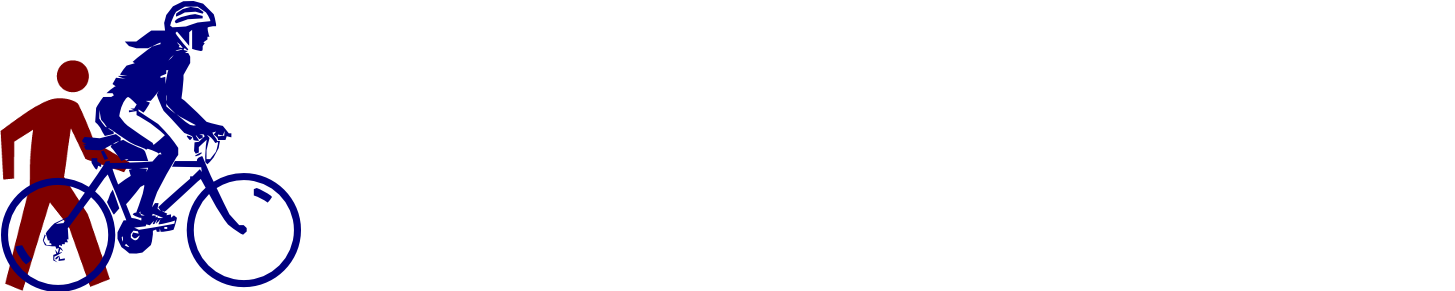
\includegraphics[width=0.5\textwidth]{x0.png}\\
	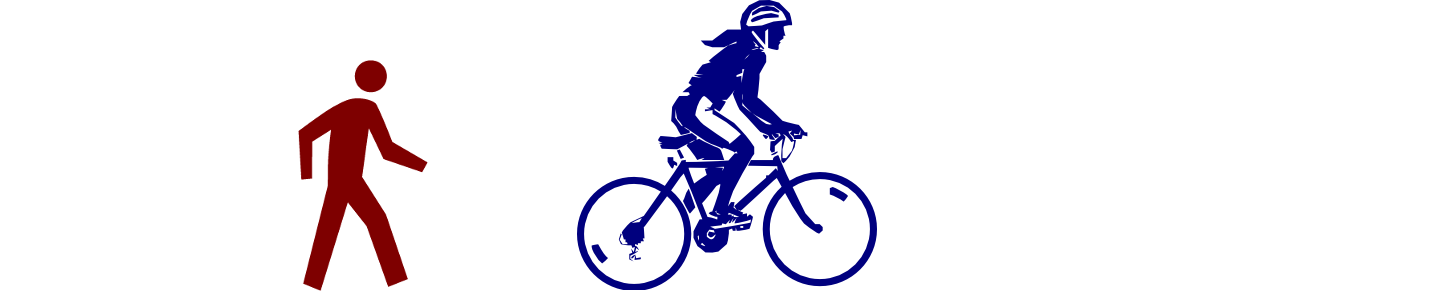
\includegraphics[width=0.5\textwidth]{x1.png}\\
	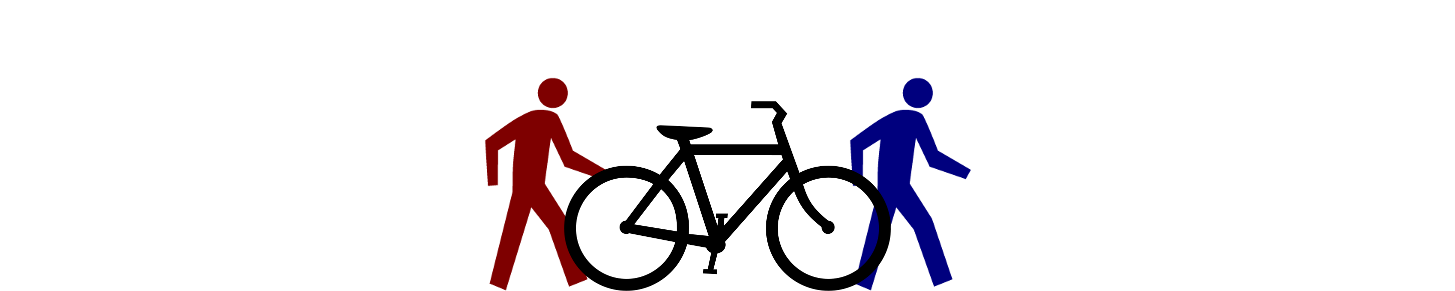
\includegraphics[width=0.5\textwidth]{x2.png}\\
	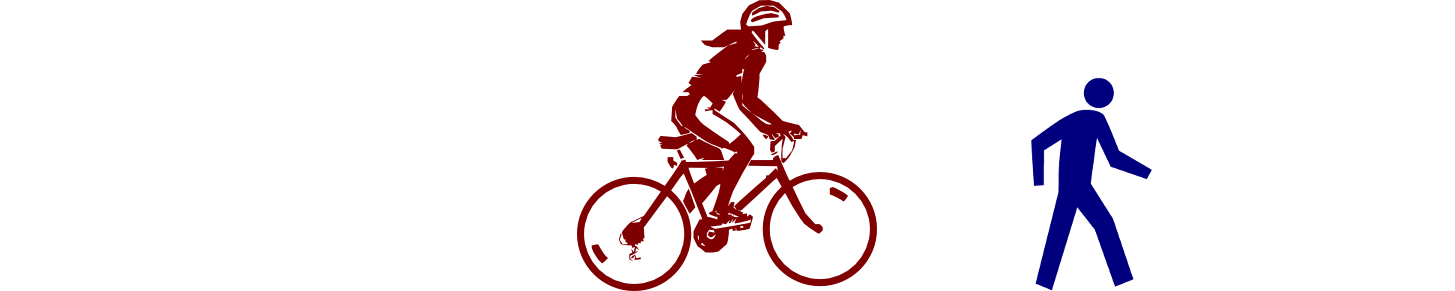
\includegraphics[width=0.5\textwidth]{x3.png}\\
	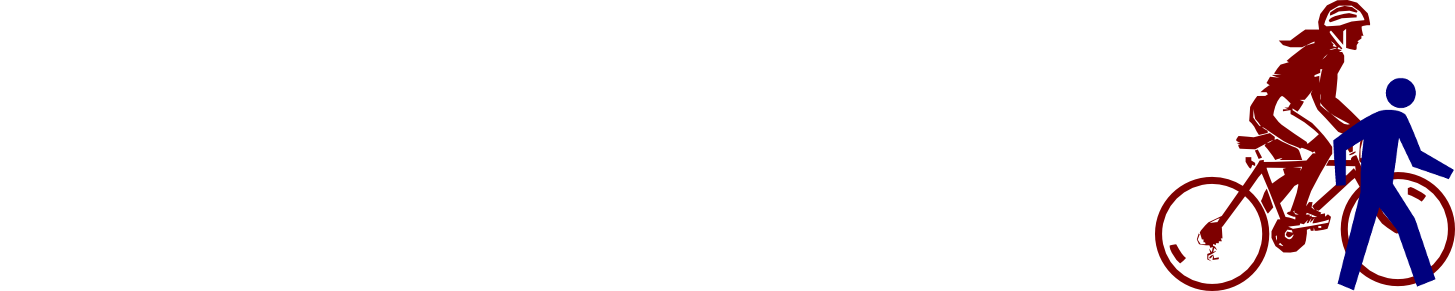
\includegraphics[width=0.5\textwidth]{x4.png}\\
	\caption{The solution for $n,k=2,1$.}
	\label{fig:sol}
\end{figure}

\initial{F}igure~\ref{fig:sol} shows the solution for 2 people sharing 1 bike.
The frames show progress after $0$, $1$, $1.5$, $2$, and $3$ units of time have elapsed, assuming $w=0.5$ and $b=1$ (i.e., biking is twice as fast as walking).
Note that the bike is idle between times $1$ and $2$ -- for a full third of the transit time! -- yet the stick figures arrive in $3$ time units, a $25\%$ improvement over walking speed, and only $50\%$ slower than both participants having a bike of their own.

\newcommand\PA{\ensuremath{\mathtt{0}}}
\newcommand\PB{\ensuremath{\mathtt{1}}}
\newcommand\PC{\ensuremath{\mathtt{2}}}
\newcommand\PD{\ensuremath{\mathtt{3}}}
\newcommand\PE{\ensuremath{\mathtt{4}}}
\newcommand\PF{\ensuremath{\mathtt{5}}}
\newcommand\PG{\ensuremath{\mathtt{6}}}
\newcommand\distance[1]{\ensuremath{\mathsf{#1}}}
Formally we say that the {\em bicycle allocation} for this case is that person \PA~(the blue one, if you're reading this electronically or printed in color) rides bike $0$ for distances between $0$ and $1$, and person \PB~(the red one, if same) rides it for distances between $1$ and $2$. For short, we write:
\begin{eqnarray*}
	p_\PA &=& b_0@0 \\
	p_\PB &=& b_0@1
\end{eqnarray*}

\subsection{Generalized It}

\initial{W}ithout loss of generality, let us say that $d$ is $n$ units of distance away (i.e., the same as the number of people).
First, some observations about the problem:
\begin{enumerate}
	\setlength{\itemsep}{-0.5em}
	\item A total of $n^2$ distances will be traveled. A total of $nk$ distances will be biked. It is pointless for bikes to go backwards.
	\item By symmetry, in an optimal solution, each person will bike $k$ distance and walk $n-k$ distance. This also means that fractional distances (less than $1/n$ of the total distance) need not be considered as places to mount/dismount.
	\item No more than $k$ people can ride for any given distance unit $[i,i+1]$. If any fewer than $k$ people rode this way, the bikes would be under-utilised. This allows us to check both validity and optimality.
	\item The optimal (minimum) total travel time is $k/b + (n-k)/w$. The optimal (maximum) average speed is $nbw/(kw+bn-bk)$.
	% TODO: Discuss epsilon.
\end{enumerate}

While Figure~\ref{fig:sol} plots the participants' positions at (time,distance) coordinates, for the general instance of the problem it is more useful to plot {\em transportation mode} (i.e., whether a person walks or rides bike $i$) at (person,distance) coordinates. For example, in Figure~\ref{fig:grids} we show $n \times n$ grids for the $2,1$; $3,2$; and $5,3$ instances of the problem.

\newcommand\BA{\cellcolor{WildStrawberry}~\textcolor{White}{$b_0$}}
\newcommand\BB{\cellcolor{NavyBlue}      ~\textcolor{White}{$b_1$}}
\newcommand\BC{\cellcolor{OliveGreen}   ~\textcolor{White}{$b_2$}}
\newcommand\BD{\cellcolor{Dandelion}    ~\textcolor{White}{$b_3$}}
\newcommand\BE{\cellcolor{ProcessBlue}       ~\textcolor{White}{$b_4$}}
\begin{figure*}[t]
	\begin{subfigure}[b]{0.28\textwidth}
		\begin{tabular}{rp{1.5em}|p{1.5em}|}
		& \multicolumn{2}{c}{distance} \\
		person & \multicolumn{1}{|c|}{\distance{0}} & \multicolumn{1}{c|}{\distance{1}} \\
		\hline
		\multicolumn{1}{r|}{\PA} & \BA & \\
		\cline{2-3}
		\multicolumn{1}{r|}{\PB} & & \BA \\
		\cline{2-3}
		\multicolumn{3}{c}{}\\
		\multicolumn{3}{c}{}\\
		\multicolumn{3}{c}{}\\
		\end{tabular}
		\caption{$2$ people, $1$ bike.}
	\end{subfigure}
	\begin{subfigure}[b]{0.33\textwidth}
		\begin{tabular}{rp{1.5em}|p{1.5em}|p{1.5em}|}
		& \multicolumn{3}{c}{distance} \\
		person & \multicolumn{1}{|c|}{\distance{0}} & \multicolumn{1}{c|}{\distance{1}} & \multicolumn{1}{c|}{\distance{2}} \\
		\hline
		\multicolumn{1}{r|}{\PA} & \BA & \BB & \\
		\cline{2-4}
		\multicolumn{1}{r|}{\PB} & & \BA & \BB \\
		\cline{2-4}
		\multicolumn{1}{r|}{\PC} & \BB & & \BA \\
		\cline{2-4}
		\multicolumn{4}{c}{}\\
		\multicolumn{4}{c}{}\\
		\end{tabular}
		\caption{$3$ people, $2$ bikes.}
	\end{subfigure}
	\begin{subfigure}[b]{0.38\textwidth}
		\begin{tabular}{rp{1.5em}|p{1.5em}|p{1.5em}|p{1.5em}|p{1.5em}|}
		& \multicolumn{5}{c}{distance} \\
		person & \multicolumn{1}{|c|}{\distance{0}} & \multicolumn{1}{c|}{\distance{1}} & \multicolumn{1}{c|}{\distance{2}} & \multicolumn{1}{c|}{\distance{3}} & \multicolumn{1}{c|}{\distance{4}} \\
		\hline
		\multicolumn{1}{r|}{\PA} &\BA&\BB&\BC&   & \\
		\cline{2-6}
		\multicolumn{1}{r|}{\PB} &   &\BA&\BB&\BC& \\
		\cline{2-6}
		\multicolumn{1}{r|}{\PC} &   &   &\BA&\BB&\BC\\
		\cline{2-6}
		\multicolumn{1}{r|}{\PD} &\BC&   &   &\BA&\BB\\
		\cline{2-6}
		\multicolumn{1}{r|}{\PE} &\BB&\BC&   &   &\BA\\
		\cline{2-6}
		\end{tabular}
		\caption{$5$ people, $3$ bikes.}
	\end{subfigure}
	\caption{Bicycle allocation policies for selected instances of the \prob. White cells represent walking; cells of different colours represent different bikes.
		Can you spot the French flag?}
	\label{fig:grids}
\end{figure*}

The pattern is now evident: Person $i$ rides a bike between distance $i$ and distance $i+k~\mathsf{mod}~n$.
To express this in the notation from the previous section, we can say: $\forall i,j$ with $0\le i < n$ and $0 \le j < k$:
\begin{eqnarray*}
	p_i  &=& b_j @ (i+j~\mathsf{mod}~n)
\end{eqnarray*}

We now show that this strategy is both possible and optimal.

\newtheorem{theorem}{Theorem}

\begin{theorem}[Optimality]
The \prob~is solved optimally when $p_i$ rides between distance $i$ and distance $i+k~\mathsf{mod}~n$.
\end{theorem}
\begin{proof}
By condition (3) above, it suffices to show that, at each distance unit, exactly $k$ people ride. A simple induction on $k$ will do nicely.
\end{proof}

\subsection{Minimizing Mounts/Dismounts}

\initial{T}he astute reader will note that, while the allocations in the above tables successfully minimize total travel time, they {\em maximize} the number of times each rider must mount and dismount a bicycle. If we let $\epsilon$ (the time to mount or dismount) be non-negligible, we see that the travel time achieved above is actually: $k/b+(n-k)/w + 2k\epsilon$.

\begin{figure}[b]
		\begin{center}
		\begin{tabular}{rp{1.5em}|p{1.5em}|p{1.5em}|p{1.5em}|p{1.5em}|}
		& \multicolumn{5}{c}{distance} \\
		person & \multicolumn{1}{|c|}{\distance{0}} & \multicolumn{1}{c|}{\distance{1}} & \multicolumn{1}{c|}{\distance{2}} & \multicolumn{1}{c|}{\distance{3}} & \multicolumn{1}{c|}{\distance{4}} \\
		\hline
		\multicolumn{1}{r|}{\PA} &\BA&\BA&\BA&   & \\
		\cline{2-6}
		\multicolumn{1}{r|}{\PB} &   &\BB&\BB&\BB& \\
		\cline{2-6}
		\multicolumn{1}{r|}{\PC} &   &   &\BC&\BC&\BC\\
		\cline{2-6}
		\multicolumn{1}{r|}{\PD} &\BB&   &   &\BA&\BA\\
		\cline{2-6}
		\multicolumn{1}{r|}{\PE} &\BC&\BC&   &   &\BB\\
		\cline{2-6}
		\end{tabular}
		\end{center}
		\caption{Each person mounts/dismounts 2 or 4 times.}
		\label{fig:continuous}
\end{figure}

We might instead attempt to allocate bicycles contiguously, like in Figure~\ref{fig:continuous} below.
Here, $n-k+1$ riders can ride ``monogamously'', though $k-1$ people will have two riding  sessions with a walking intermission. This gives us a better travel time of $k/b+(n-k)/w + 4\epsilon$, which is a strict improvement whenever $k>2$.

\begin{theorem}[Contiguous Allocation]
\label{thm:cont}
For all $n$ and $k$, an optimal bicycle allocation exists in which no rider mounts and dismounts more than four times, and is given as follows:
\newcommand\open{\{}
\newcommand\close{\}}
\begin{center}
\begin{tabular}{rclll}
	$p_i$ & $=$ & $b_{(i~\mathsf{mod}~k)}@ \open i \rightsquigarrow i+k \close$ && $i \le n-k$ \\
	\\
	\multirow{2}{*}{$p_i$} & \multirow{2}{*}{$=$} & $b_{(i~\mathsf{mod}~k)}@ \open i\rightsquigarrow n \close,$ && \multirow{2}{*}{$i > n-k$} \\
	& & $b_{(i+k-n)}\hspace{0.5em}@ \open 0 \rightsquigarrow i+k-n \close$ \\
	\\
\end{tabular}
\end{center}
where $b_x@\open y\rightsquigarrow z\close$ expands to $b_x@(y)$, $b_x@(y+1)$, \dots $b_x@(z-1)$.

\end{theorem}
\begin{proof}
By induction on $k$.
\end{proof}


\section{Evaluation}

\initial{I}n Figure~\ref{fig:graph} we find our visualizings.
The horizontal line on top represents the previous state of the art, in which some participants walk the entire distance.
The bottom line represents the ideal case, in which there are enough bikes for everyone to ride together.

Here we have plotted the travel time for various values of $n,k$ against different configurations of the $b/w$ ratio; i.e., how much faster it is to bike than to walk.
We hope this presentation will be useful in many different terrains; for example, if the destination is downhill, $b/w$ may be very high indeed.

\section{Conclusion}

\initial{Y}ou and your friends have arrived at $d$ at the unprecedentedly fast speed of $nbw/(kw+bn-bk)$, and are warming up indoors and enjoying dinner. ``Wow,'' you say, ``I sure am glad everyone thought to make $n$ copies of their bike-lock keys!''


\begin{figure*}[t]
	\centering
	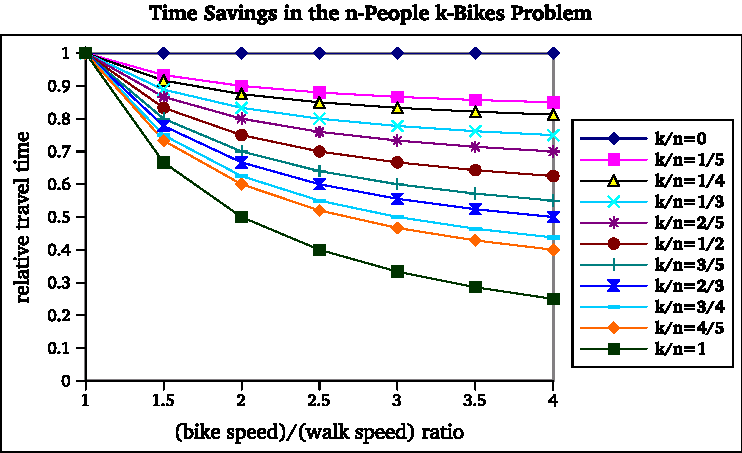
\includegraphics[width=0.85\textwidth]{graph.pdf}
	\caption{Speedup achieved in the \prob. As always, lower is better.}
	\label{fig:graph}
\end{figure*}
%----------------------------------------------------------------------------------------
%	REFERENCE LIST
%----------------------------------------------------------------------------------------

\bibliographystyle{abbrv}
\bibliography{bikes}

%----------------------------------------------------------------------------------------

\newpage
\appendix
\section{Scratch Work}

These are some more tables we drew when deciding whether Theorem~\ref{thm:cont} was even true at all, and they were too colorful not to include.

\begin{figure}[h]
		\begin{center}
		%	\begin{tabular}{rp{1.5em}|p{1.5em}|p{1.5em}|p{1.5em}|p{1.5em}|p{1.5em}|}
		%& \multicolumn{6}{c}{distance} \\
		%person & \multicolumn{1}{|c|}{\distance{0}} & \multicolumn{1}{c|}{\distance{1}} & \multicolumn{1}{c|}{\distance{2}} & \multicolumn{1}{c|}{\distance{3}} & \multicolumn{1}{c|}{\distance{4}} & \multicolumn{1}{c|}{\distance{5}} \\
		%\hline
		%\multicolumn{1}{r|}{\PA} &\BA&\BA&\BA&\BA&   &   \\
		%\cline{2-7}
		%\multicolumn{1}{r|}{\PB} &   &\BB&\BB&\BB&\BB&   \\
		%\cline{2-7}
		%\multicolumn{1}{r|}{\PC} &   &   &\BC&\BC&\BC&\BC\\
		%\cline{2-7}
		%\multicolumn{1}{r|}{\PD} &\BB&   &   &\BD&\BD&\BD\\
		%\cline{2-7}
		%\multicolumn{1}{r|}{\PE} &\BC&\BC&   &   &\BA&\BA\\
		%\cline{2-7}
		%\multicolumn{1}{r|}{fff} &\BD&\BD&\BD&   &   &\BB\\
		%\cline{2-7}
		%\end{tabular}
		%% 6/4
		%	\begin{tabular}{rp{1.5em}|p{1.5em}|p{1.5em}|p{1.5em}|p{1.5em}|p{1.5em}|}
		%& \multicolumn{6}{c}{distance} \\
		%person & \multicolumn{1}{|c|}{\distance{0}} & \multicolumn{1}{c|}{\distance{1}} & \multicolumn{1}{c|}{\distance{2}} & \multicolumn{1}{c|}{\distance{3}} & \multicolumn{1}{c|}{\distance{4}} & \multicolumn{1}{c|}{\distance{5}} \\
		%\hline
		%\multicolumn{1}{r|}{\PA} &\BA&\BA&\BA&\BA&\BA&   \\
		%\cline{2-7}
		%\multicolumn{1}{r|}{\PB} &   &\BB&\BB&\BB&\BB&\BB\\
		%\cline{2-7}
		%\multicolumn{1}{r|}{\PC} &\BB&   &\BC&\BC&\BC&\BC\\
		%\cline{2-7}
		%\multicolumn{1}{r|}{\PD} &\BC&\BC&   &\BD&\BD&\BD\\
		%\cline{2-7}
		%\multicolumn{1}{r|}{\PE} &\BD&\BD&\BD&   &\BE&\BE\\
		%\cline{2-7}
		%\multicolumn{1}{r|}{fff} &\BE&\BE&\BE&\BE&   &\BA\\
		%\cline{2-7}
		%\end{tabular}
		% 7/3
		\begin{tabular}{rp{1.5em}|p{1.5em}|p{1.5em}|p{1.5em}|p{1.5em}|p{1.5em}|p{1.5em}|}
			& \multicolumn{7}{c}{distance} \\
			person & \multicolumn{1}{|c|}{\distance{0}} & \multicolumn{1}{c|}{\distance{1}} & \multicolumn{1}{c|}{\distance{2}} & \multicolumn{1}{c|}{\distance{3}} & \multicolumn{1}{c|}{\distance{4}} & \multicolumn{1}{c|}{\distance{5}} & \multicolumn{1}{c|}{\distance{6}}\\
			\hline
			\multicolumn{1}{r|}{\PA} &\BA&\BA&\BA&   &   &   &   \\
			\cline{2-8}
			\multicolumn{1}{r|}{\PB} &   &\BB&\BB&\BB&   &   &   \\
			\cline{2-8}
			\multicolumn{1}{r|}{\PC} &   &   &\BC&\BC&\BC&   &   \\
			\cline{2-8}
			\multicolumn{1}{r|}{\PD} &   &   &   &\BA&\BA&\BA&   \\
			\cline{2-8}
			\multicolumn{1}{r|}{\PE} &   &   &   &   &\BB&\BB&\BB\\
			\cline{2-8}
			\multicolumn{1}{r|}{\PF} &\BB&   &   &   &   &\BC&\BC\\
			\cline{2-8}
			\multicolumn{1}{r|}{\PG} &\BC&\BC&   &   &   &   &\BA\\
			\cline{2-8}
		\end{tabular}
		\vspace{1em}

		\begin{tabular}{rp{1.5em}|p{1.5em}|p{1.5em}|p{1.5em}|p{1.5em}|p{1.5em}|p{1.5em}|}
			& \multicolumn{7}{c}{distance} \\
			person & \multicolumn{1}{|c|}{\distance{0}} & \multicolumn{1}{c|}{\distance{1}} & \multicolumn{1}{c|}{\distance{2}} & \multicolumn{1}{c|}{\distance{3}} & \multicolumn{1}{c|}{\distance{4}} & \multicolumn{1}{c|}{\distance{5}} & \multicolumn{1}{c|}{\distance{6}}\\
			\hline
			\multicolumn{1}{r|}{\PA} &\BA&\BA&\BA&\BA&\BA&   &   \\
			\cline{2-8}
			\multicolumn{1}{r|}{\PB} &   &\BB&\BB&\BB&\BB&\BB&   \\
			\cline{2-8}
			\multicolumn{1}{r|}{\PC} &   &   &\BC&\BC&\BC&\BC&\BC\\
			\cline{2-8}
			\multicolumn{1}{r|}{\PD} &\BB&   &   &\BD&\BD&\BD&\BD\\
			\cline{2-8}
			\multicolumn{1}{r|}{\PE} &\BC&\BC&   &   &\BE&\BE&\BE\\
			\cline{2-8}
			\multicolumn{1}{r|}{\PF} &\BD&\BD&\BD&   &   &\BA&\BA\\
			\cline{2-8}
			\multicolumn{1}{r|}{\PG} &\BE&\BE&\BE&\BE&   &   &\BB\\
			\cline{2-8}
		\end{tabular}
		\end{center}
		\caption{
To those who printed in black-and-white and find these illegible, we say: stop reinforcing the color binary!}
\end{figure}

\end{document}
